\documentclass{article}
\usepackage{graphicx}
\usepackage{amsmath}
\usepackage{amsfonts}
\usepackage{bookmark}
\usepackage{booktabs}
\usepackage{exercises}
\graphicspath{ {./images/test} }
\usepackage{indentfirst}
\usepackage{amsthm}
\usepackage{yhmath}
\usepackage{geometry}
\usepackage{placeins}
\usepackage{csquotes}
\usepackage{pgfplots}
\newcommand*{\oldneg}{\mathord{\sim}}
\newcommand\showdiv[1]{\overline{\smash{)}#1}}
\newcommand\Mydiv[1]{%
\smash{\raise.3ex\hbox{$\big)$}}\mkern-8mu
        \overline{\enspace\strut#1}}
\setlength{\tabcolsep}{5pt}
\theoremstyle{definition}
\newtheorem{definition}{Definition}

\setlength{\parindent}{.5in}
\setlength{\parskip}{12pt}
\renewcommand{\arraystretch}{2}
\geometry{margin=1in}
\newcommand{\?}{\stackrel{?}{=}}
\pgfplotsset{width=7cm,compat=1.18}\usepgfplotslibrary{statistics}

\title{Test Answers (pg. 371)}
\begin{document}
\maketitle

\section*{1}
$y=\frac{a}{x}$ and $2=\frac{a}{5}$ meaning $a=10$. Thus, when $x=4$, 
$y=\frac{10}{4}=\frac{5}{2}$.

\section*{2}
$y=\frac{a}{x}$ and $\frac{7}{2}=\frac{a}{-4}$ meaning $a=-14$. Thus, when $x=4$, $y=\frac{-14}{4}=-\frac{7}{2}$.

\section*{3}
$y=\frac{a}{x}$ and $\frac{5}{8}=\frac{a}{\frac{3}{4}}=\frac{4a}{3}$ meaning $a=\frac{15}{32}$. Thus, when $x=4$,
$y=\frac{\frac{15}{32}}{4}=\frac{15}{128}$.

\section*{4}
We know that there is a vertical asymptote of $-5$ and a horizontal asymptote of $-3$:
\newline 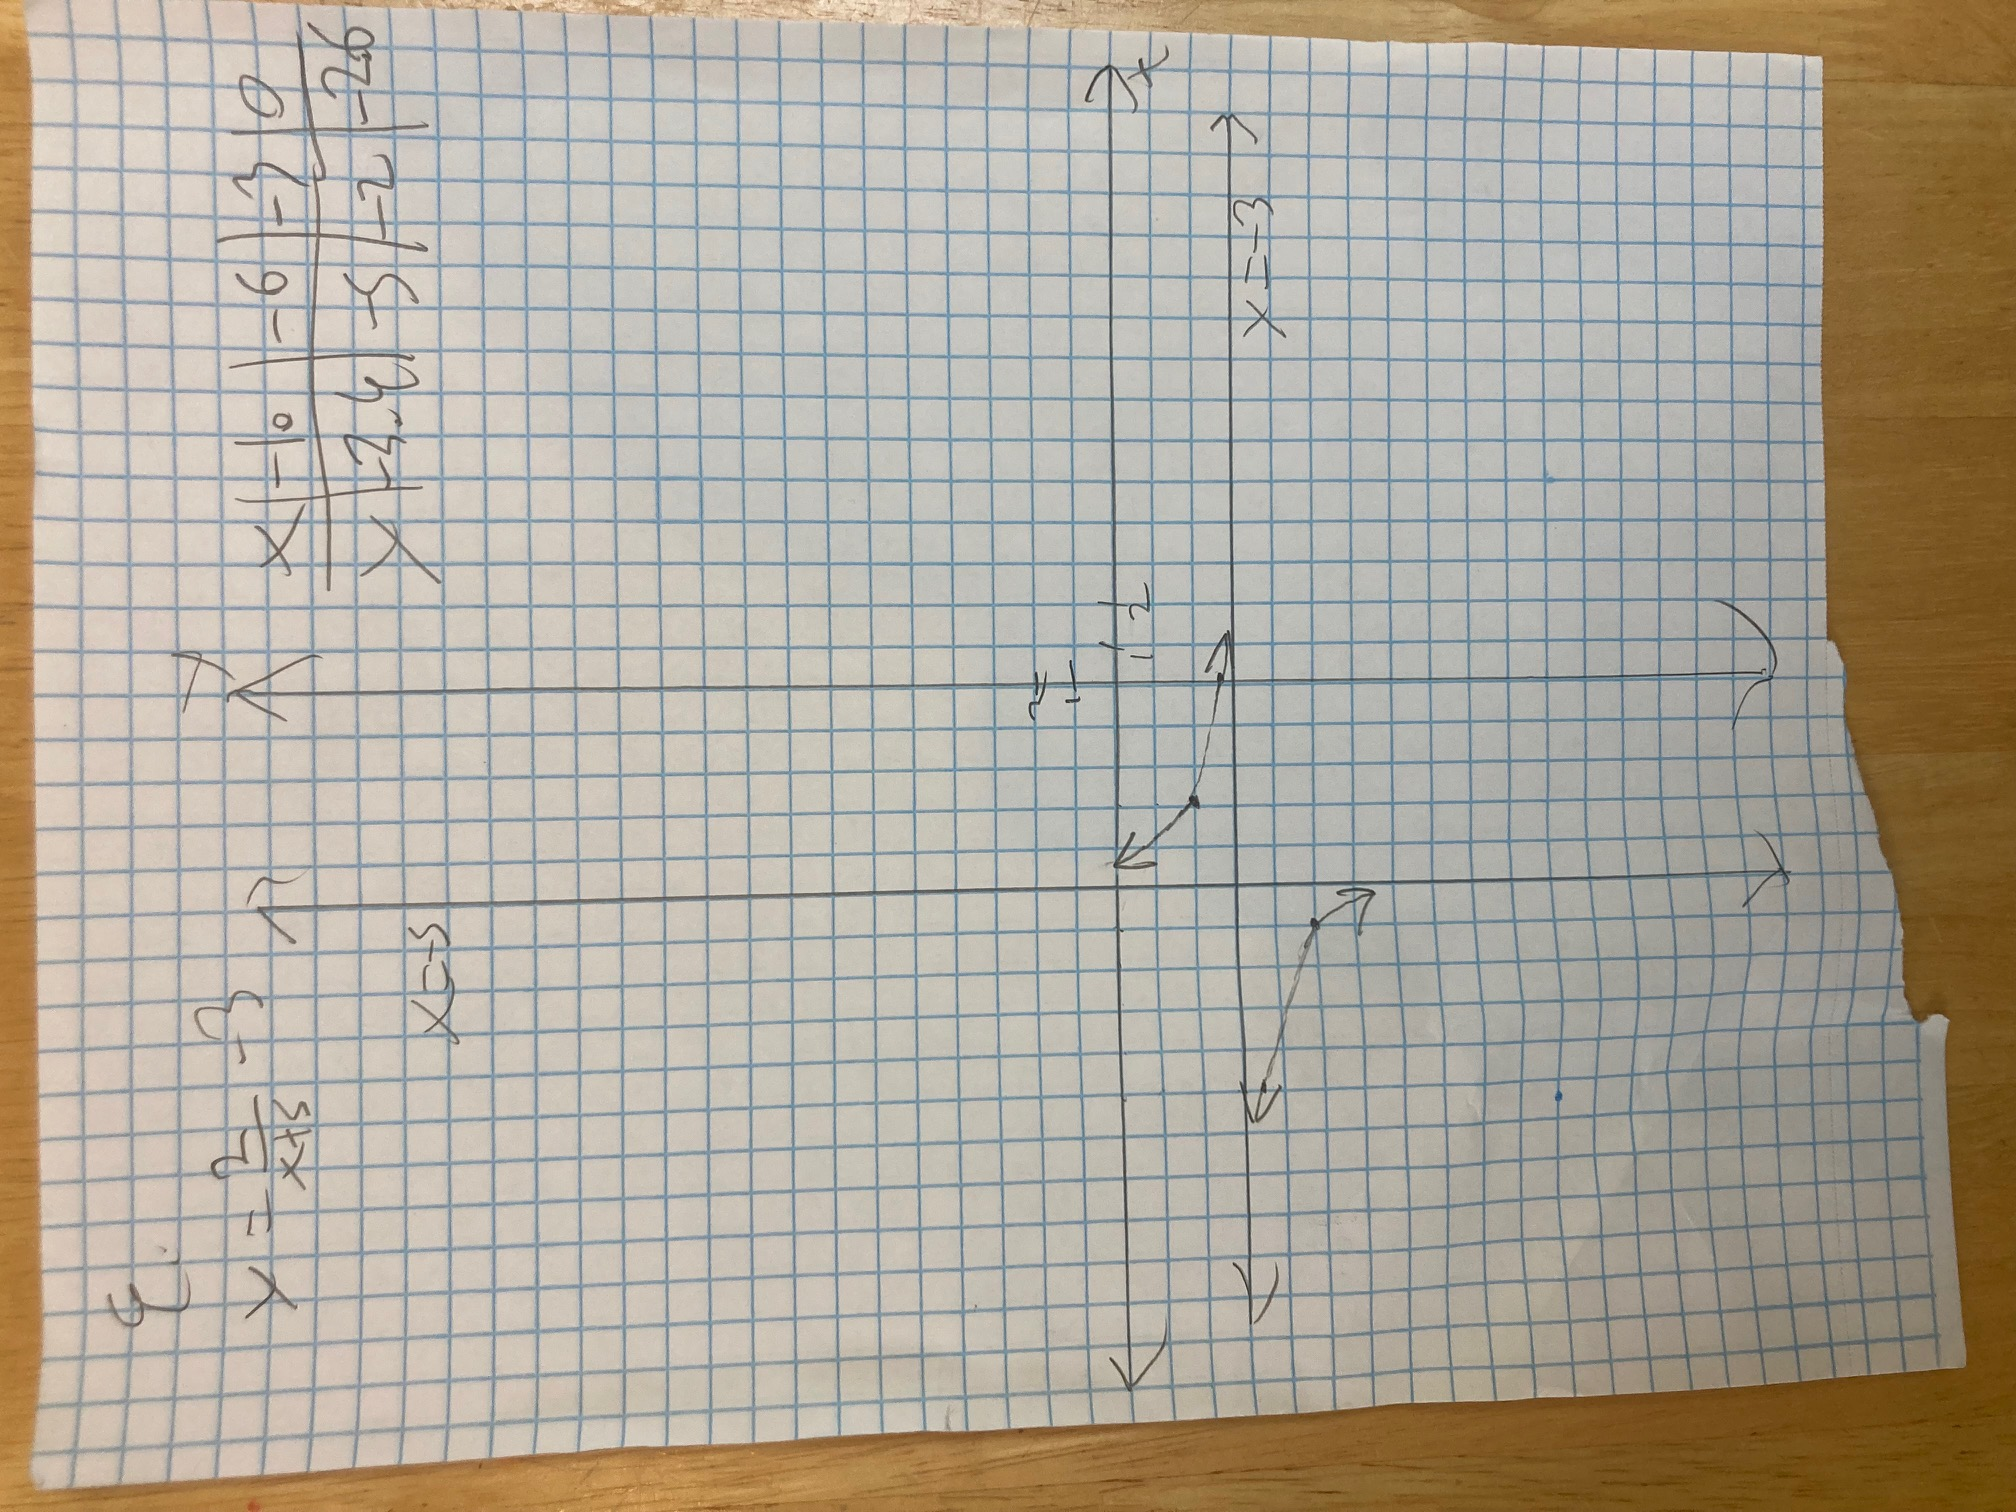
\includegraphics[width = 4in, height = 4in, angle = -90]{9}\newline

\section*{5}
We know that there is a vertical asymptote of $4$ and a horiztonal asymmptote of $-1$:
\newline 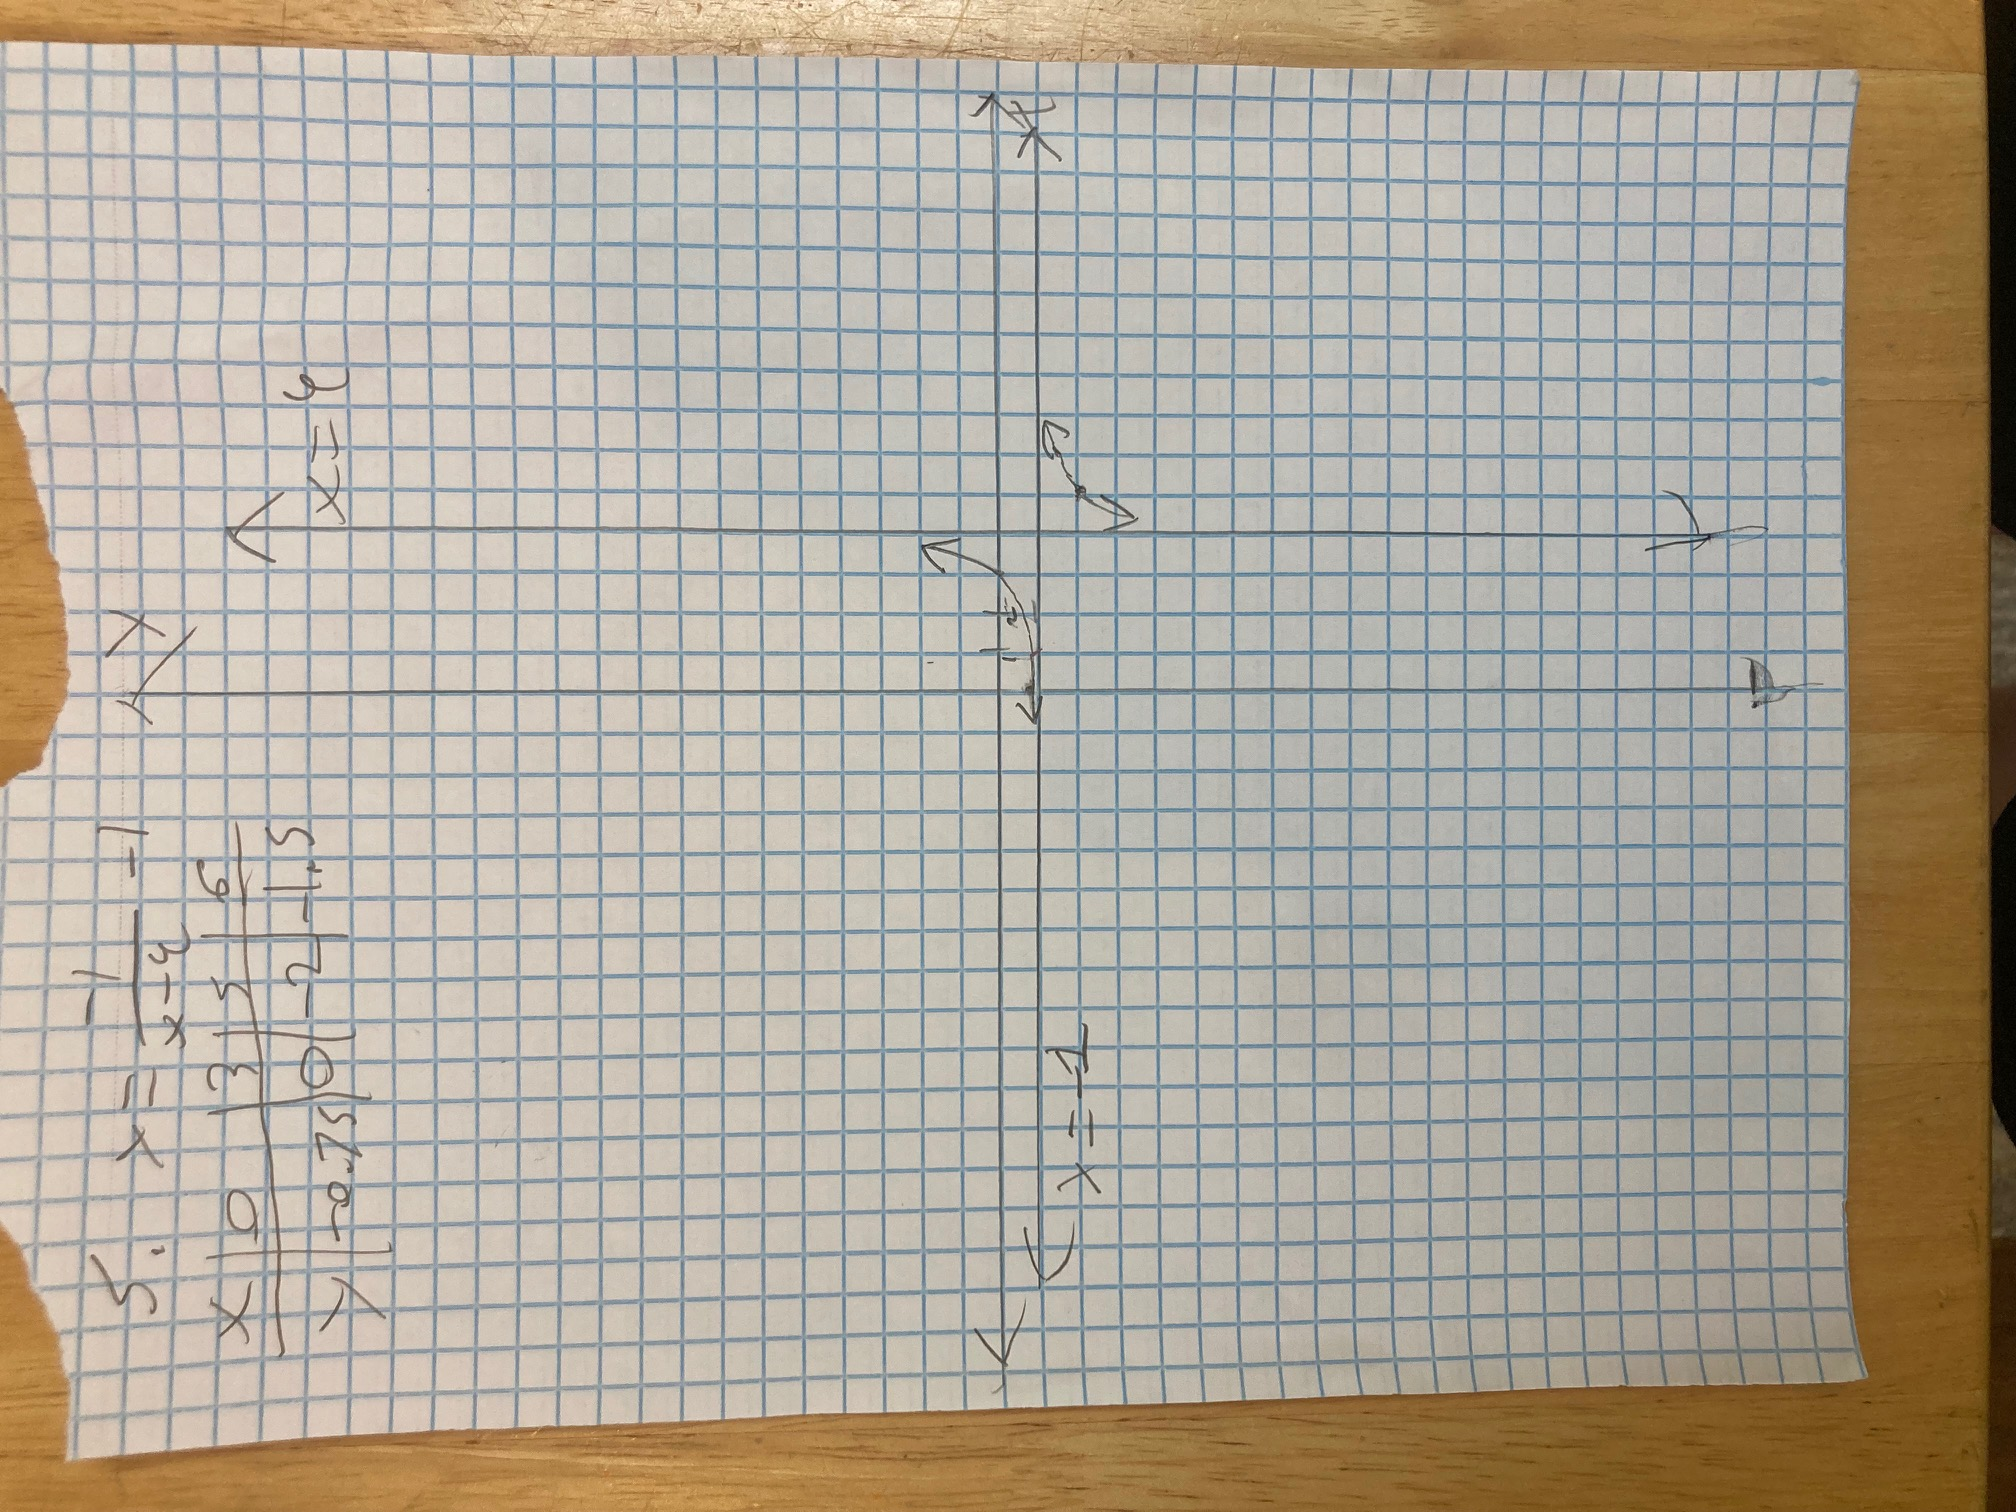
\includegraphics[width = 4in, height = 4in, angle = -90]{8}\newline

\section*{6}
Note that the solution to $6-x=0$ is $x=6$ and the solution to $2x+1=0$ is $x=-\frac{1}{2}$. Thus the $x$-intercept of the graph is 
$x=6$, the vertical asymptote is $-\frac{1}{2}$, and the horizontal asymptote is $\frac{-1}{2}=-\frac{1}{2}$:
\newline 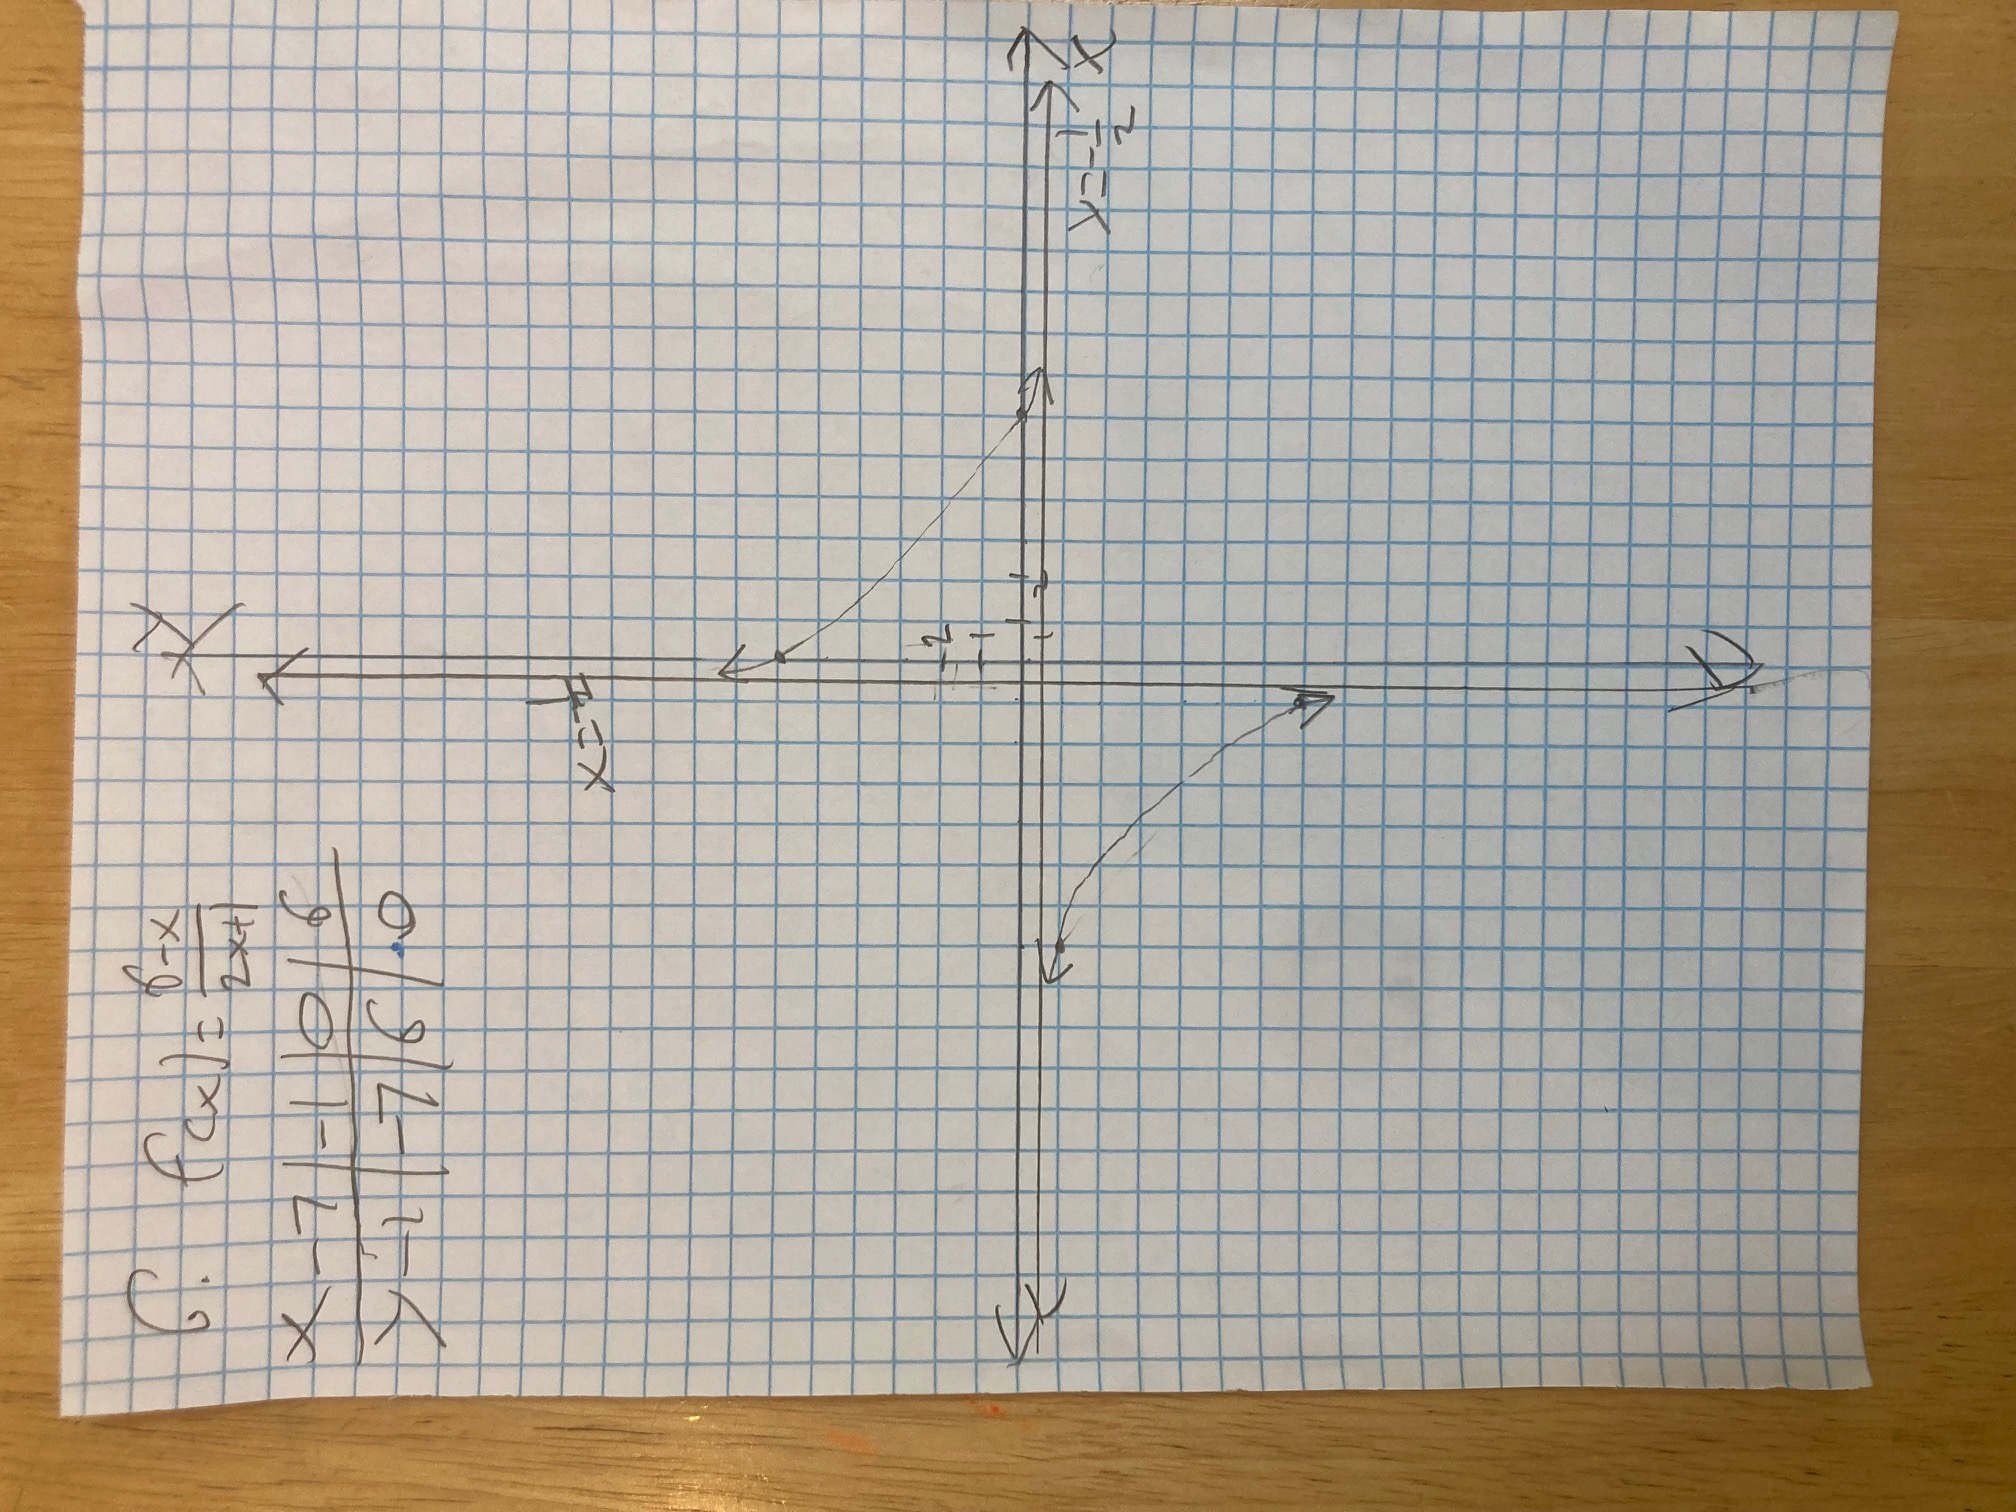
\includegraphics[width = 4in, height = 4in, angle = -90]{7}\newline

\section*{7}
Because $x^2+2=0$ has no real solutions, the graph of the function has a horizontal asymptote of $y=0$, no vertical asymptotes, and no $x$-intercepts.
\newline 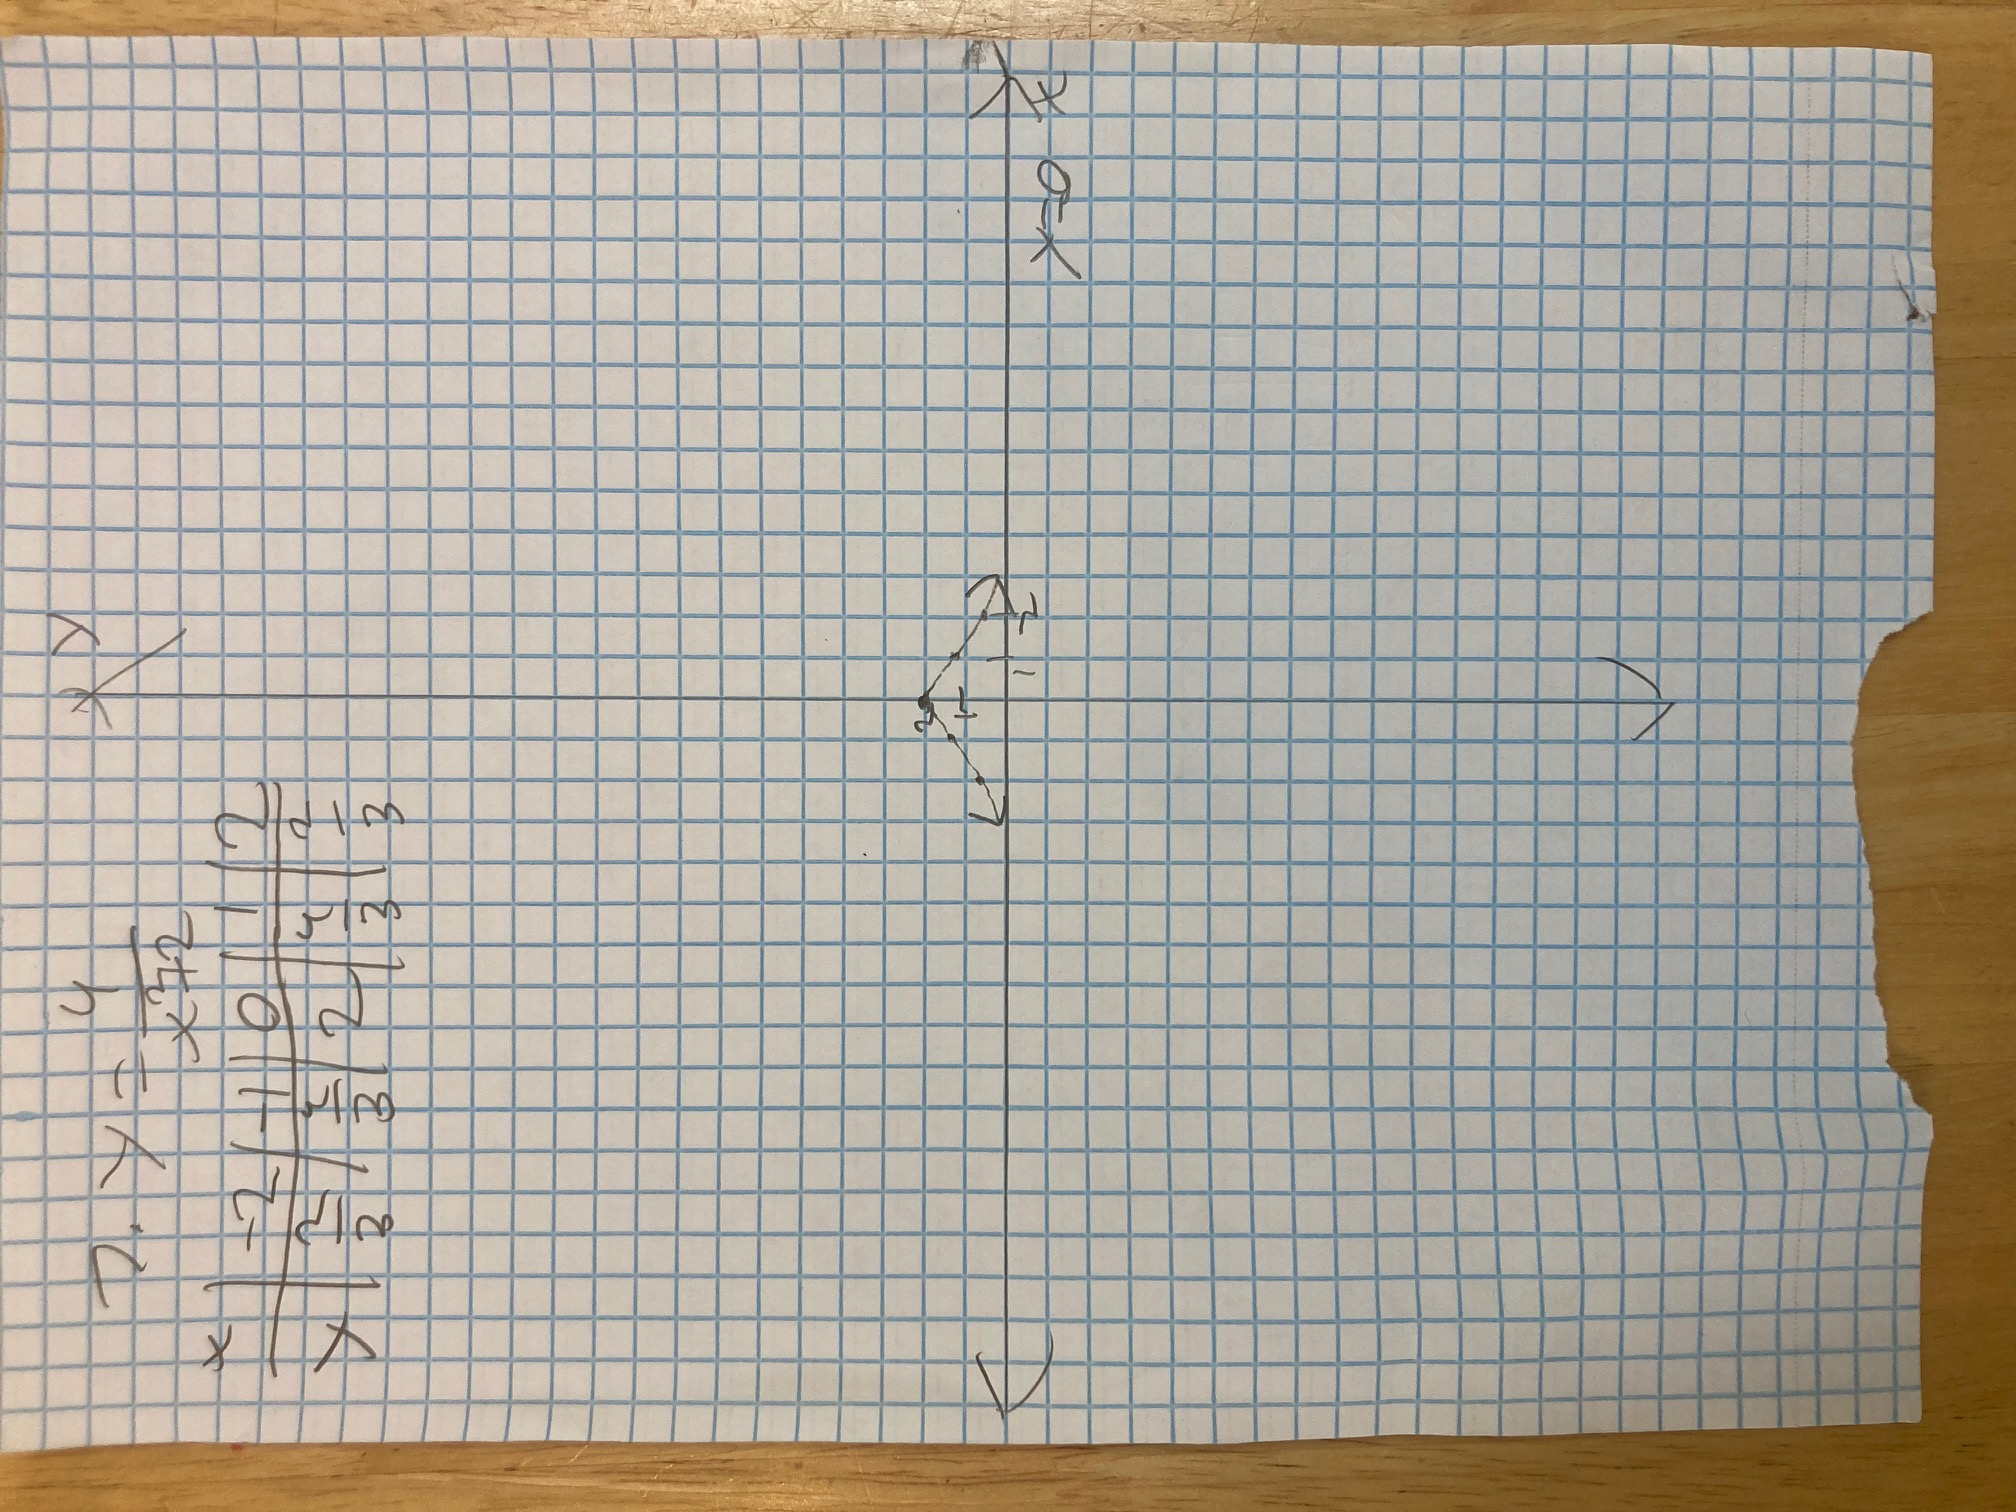
\includegraphics[width = 4in, height = 4in, angle = -90]{6}\newline

\section*{8}
Because $x^2-4=0$ has the solutions $\pm 2$, and $x^2+8x+15=(x+5)(x+3)=0$ has the solutions $x=-5$ and $x=-3$, the graph of the function has 
a horizontal asymptote of $y=\frac{1}{1}=1$, vertical asymptotes of $x=-5$ and $x=-3$, and $x$-intercepts of $\pm 2$:
\newline 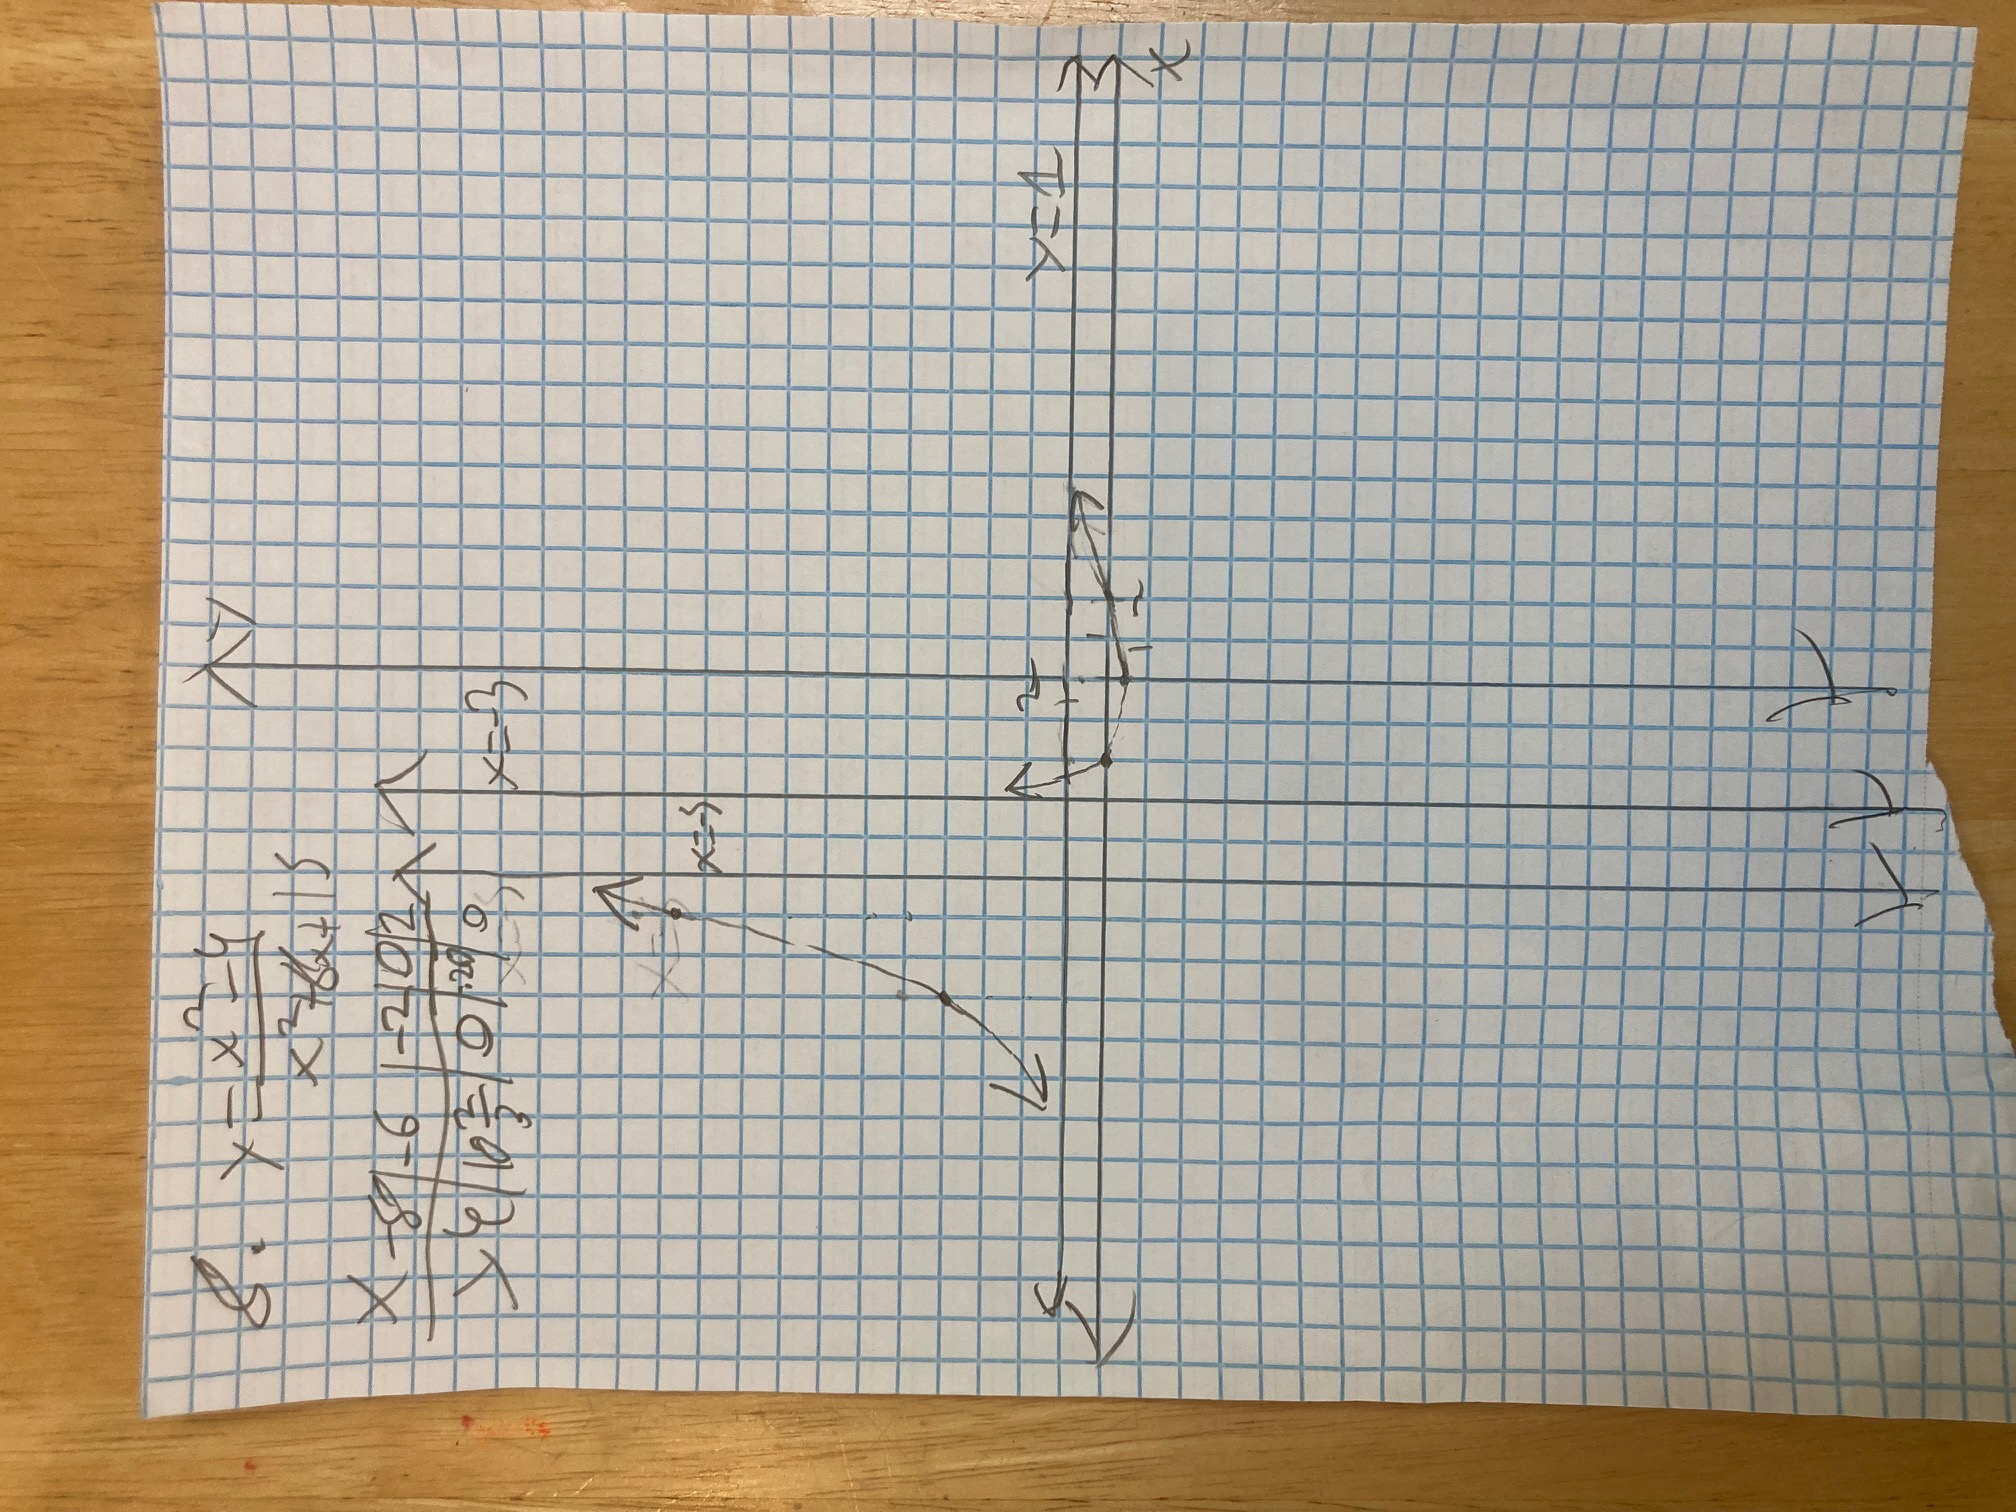
\includegraphics[width = 4in, height = 4in, angle = -90]{5}\newline

\section*{9}
Because $x^2+3=0$ has no real solutions, and $2x-1$ has the solution $x=\frac{1}{2}$, the graph of the function has 
no horizontal asymptote, no $x$-intercepts, and a vertical asymptote of $x=\frac{1}{2}$. In addition, the end behavior of the graph is the same as that of the 
graph $\frac{1}{2}x$, for which $x\rightarrow -\infty$ as $x\rightarrow -\infty$ and $x\rightarrow +\infty$ as $x\rightarrow +\infty$:
\newline 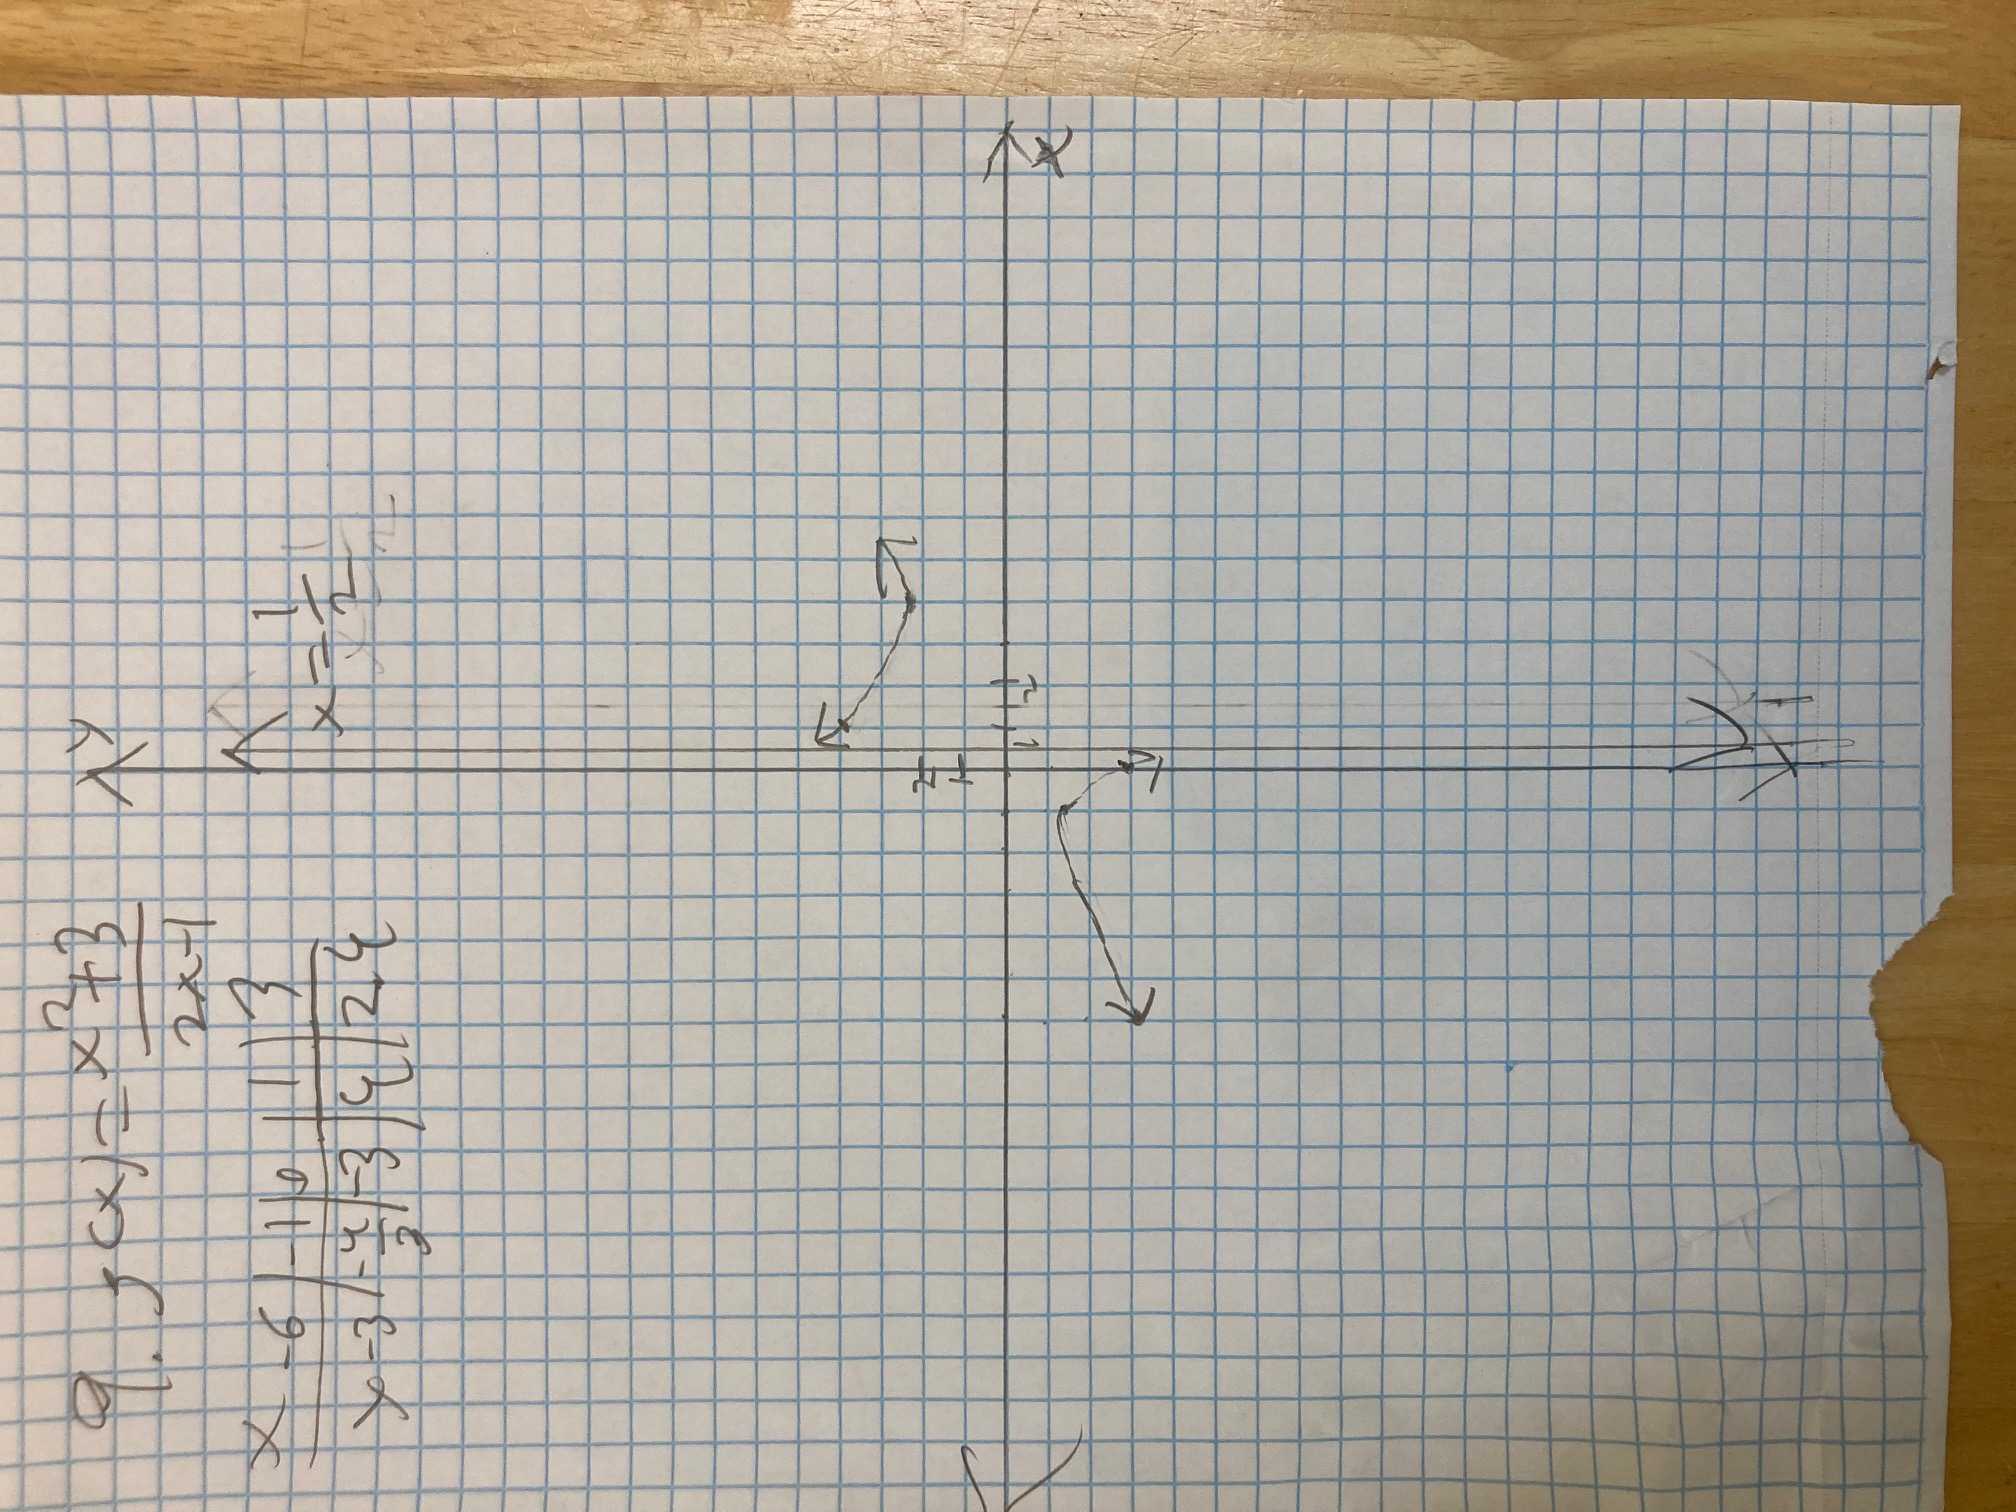
\includegraphics[width = 4in, height = 4in, angle = -90]{4}\newline

\section*{10}
$x(x-3)(x+5)$

\section*{11}
$8x^2(x-2)(x+2)$

\section*{12}
The LCM of $x^2-4x=x(x-4)$ and $x^2-2x-8=(x-4)(x+2)$ is $x(x-4)(x+2)$.

\section*{13}
The LCM of $2x+6=2(x+3)$ and $x^3+10x^2+21x=x(x^2+10x+21)=x(x+7)(x+3)$ is $2x(x+7)(x+3)$.

\section*{14}
\[ \dfrac{3x^2y}{4x^3y^5}\div\dfrac{6y^2}{2xy^3}=\dfrac{3x^2y}{4x^3y^5}\times\dfrac{2xy^3}{6y^2} \]
\[ =\dfrac{6x^3y^4}{24x^3y^7}=\dfrac{1}{4y^3} \]

\section*{15}
\[ \dfrac{x^2-3x-4}{x^2-3x-18}\times\dfrac{x-6}{x+1}=\dfrac{(x-4)(x+1)}{(x-6)(x+3)}\times\dfrac{x-6}{x+1} \]
\[ =\dfrac{(x-4)(x+1)(x-6)}{(x-6)(x+3)(x+1)}=\dfrac{x-4}{x+3} \]

\section*{16}
\[ \dfrac{x^2-8x+15}{x^2+12x+32}\times\dfrac{x+4}{x^2-25}=\dfrac{(x-5)(x-3)}{(x+8)(x+4)}\times\dfrac{x+4}{(x+5)(x-5)} \]
\[ =\dfrac{(x-5)(x-3)(x+4)}{(x+8)(x+4)(x+5)(x-5)}=\dfrac{x-3}{(x+8)(x+5)} \]

\section*{17}
\[ \dfrac{x^2-11x+28}{x^2+5x+4}\div(x^2-16)=\dfrac{(x-7)(x-4)}{(x+4)(x+1)}\times\frac{1}{(x+4)(x-4)} \]
\[ =\dfrac{(x-7)(x-4)}{(x+4)(x+1)(x+4)(x-4)}=\dfrac{x-7}{(x+4)^2(x+1)} \]

\section*{18}
\[ \dfrac{3x}{x^2+x-12}-\dfrac{6}{x+4}=\dfrac{3x}{(x+4)(x-3)}-\dfrac{6}{x+4} \]
\[ =\dfrac{3x}{(x+4)(x-3)}-\dfrac{6(x-3)}{(x+4)(x-3)}=\dfrac{3x-6(x-3)}{(x+4)(x-3)} \]
\[ =\dfrac{-3x+18}{(x+4)(x-3)}=\dfrac{-3(x-6)}{(x+4)(x-3)} \]

\section*{19}
\[ \dfrac{4}{x+5}+\dfrac{2x}{x^2-25}=\dfrac{4}{x+5}+\dfrac{2x}{(x+5)(x-5)} \]
\[ =\dfrac{4(x-5)}{(x+5)(x-5)}+\dfrac{2x}{(x+5)(x-5)} \]
\[ =\dfrac{4(x-5)+2x}{(x+5)(x-5)}=\dfrac{2(3x-10)}{(x+5)(x-5)} \]

\section*{20}
\[ \frac{3}{x+2}=\frac{x-3}{2x+4} \]
\[ 6x+12=x^2-x-6 \] \[ x^2-7x-18=0 \] \[ (x-9)(x+2)=0 \] \[ x=9\vee x=-2 \]
Check for extraneous solutions:
\[ \frac{3}{9+2}\?\frac{9-3}{2(9)+4} \] \[ \frac{3}{11}=\frac{3}{11} \]
and \[ \frac{3}{-2+2}\?\frac{-2-3}{2(-2)+4} \] which is impossible, as we cannot divide by $-2+2=0$. Thus $x=9$ is the only solution.

\section*{21}
\[ \frac{1}{x+6}+\frac{x+1}{x}=\frac{13}{x+6} \]
\[ x(x+6)(\frac{1}{x+6}+\frac{x+1}{x})=\frac{13}{x+6}x(x+6) \]
\[ x+(x+6)(x+1)=13x \] \[ x^2-5x+6=0 \] \[ (x-3)(x-2)=0 \] \[ x=3\vee x=2 \]
Check for extraneous solutions:
\[ \frac{1}{3+6}+\frac{3+1}{3}\?\frac{13}{3+6} \] \[ \frac{1}{9}+\frac{4}{3}\?\frac{13}{9} \] \[ \frac{13}{9}=\frac{13}{9} \]
and \[ \frac{1}{2+6}+\frac{2+1}{2}\?\frac{13}{2+6} \] \[ \frac{1}{8}+\frac{3}{2}\?\frac{13}{8} \] \[ \frac{13}{8}=\frac{13}{8} \]
meaning both $x=3$ and $x=2$ are solutions.

\section*{22}
\[ \frac{x-2}{x-1}=\frac{x+2}{x+4} \] \[ (x-1)(x+4)\frac{x-2}{x-1}=\frac{x+2}{x+4}(x-1)(x+4) \]
\[ (x+4)(x-2)=(x+2)(x-1) \] \[ x^2+2x-8=x^2+x-2 \] \[ x-6=0 \] \[ x=6 \]
Check for extraneous solutions:
\[ \frac{6-2}{6-1}\?\frac{6+2}{6+4} \] \[ \frac{4}{5}=\frac{4}{5} \]
meaning $x=6$ is the solution.

\section*{23}
We are asked to find the average rate of change for the function $f(x)=4^{x-3}$ over four given intervals:\newline
$[3,4]$: $\dfrac{4^{3-3}-4^{4-3}}{3-4}=3$\newline
$[4,5]$: $\dfrac{4^{4-3}-4^{5-3}}{4-5}=12$\newline
$[5,6]$: $\dfrac{4^{5-3}-4^{6-3}}{5-6}=48$\newline
$[6,7]$: $\dfrac{4^{6-3}-4^{7-3}}{6-7}=192$\newline
From these examples, we can see that the average rate of change of $x$ increases by a factor of $4$ from each interval to the next. Thus, as $x$ increases, the 
average rate of change also increases. This means that the graph of $f(x)$ will, as $x$ increases, rise more rapidly over time.

\section*{24}
$I=\frac{a}{r^2}$

\section*{25}
We know that the one-time fee is \$30, and the montly fee is \$50. Thus, after $x$ months, the fee will be $50x+30$. Hence the function for the average cost per month 
is $f(x)=\frac{50x+30}{x}$
\newline 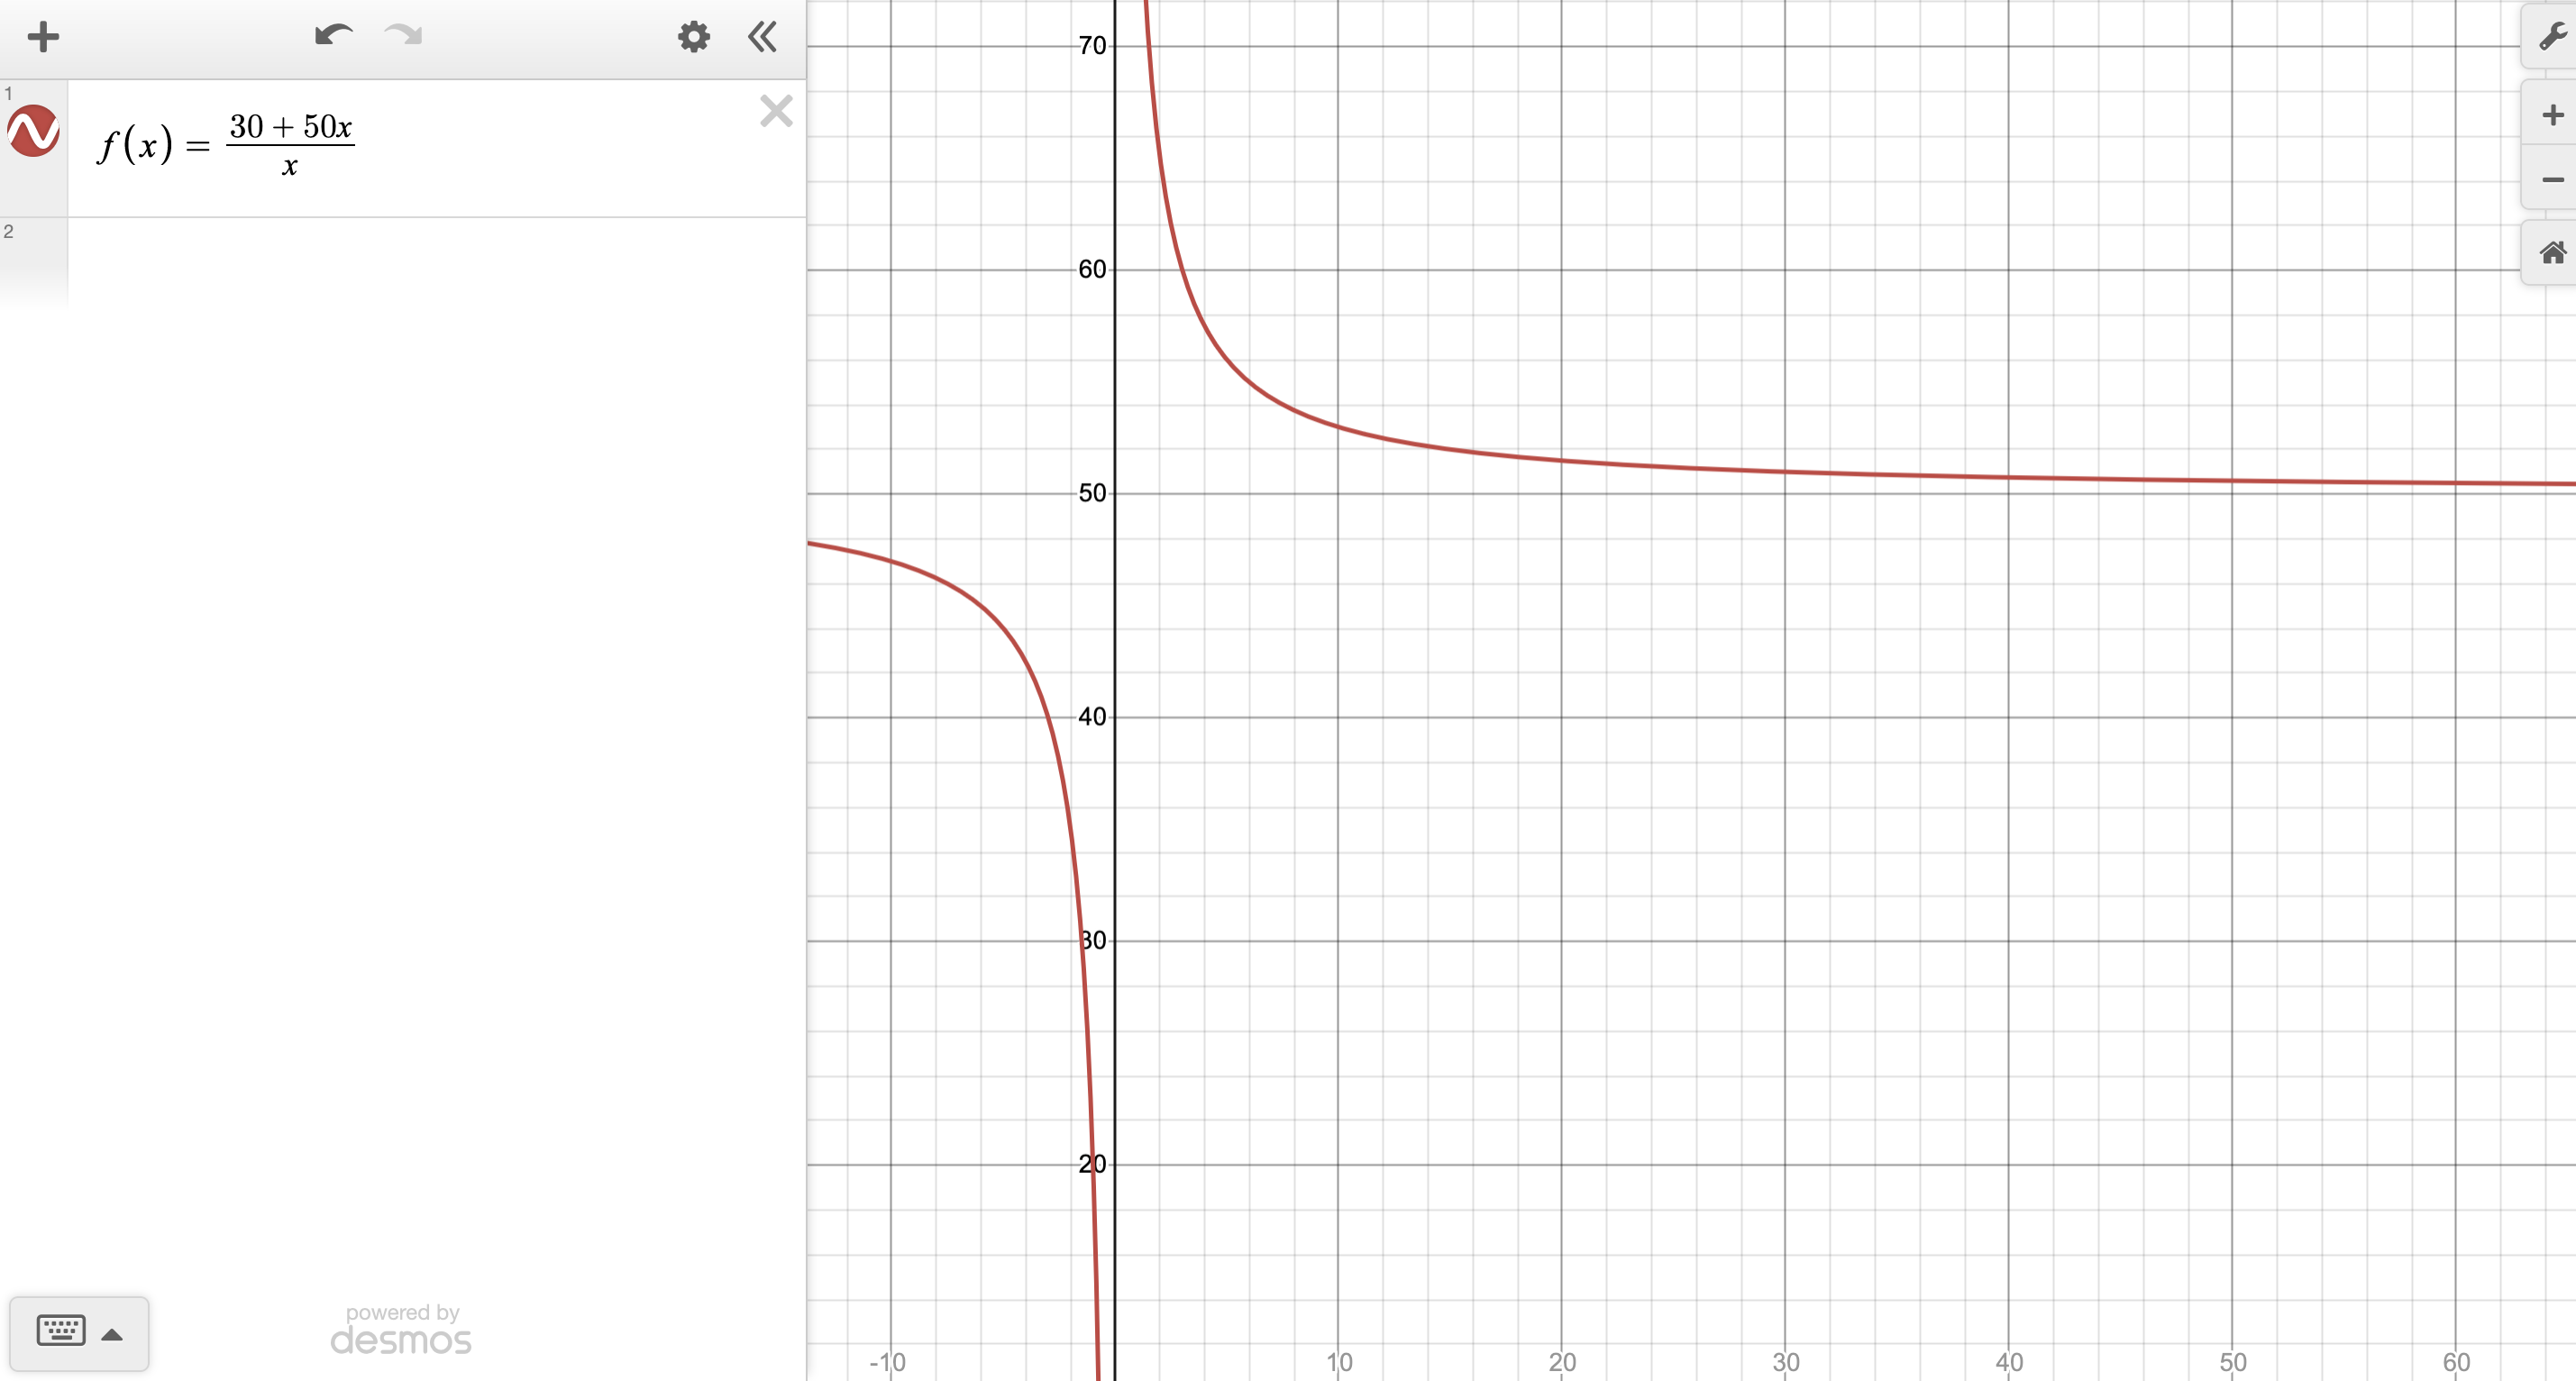
\includegraphics[width = 4in, height = 4in]{25}\newline


To reach an average cost per month of $\$56$, we solve the following equation:
\[ 56=\frac{50x+30}{x} \] \[ 56x=50x+30 \] \[ 6x=30 \] \[ x=5 \]
Check for extraneous solutions:
\[ 56\?\frac{50(5)+30}{5} \] \[ 56=56 \] Thus the average cost will be $\$56$ per month after 5 months.

\section*{26}
We know that the one-time fee is \$50, and the monthly fee is \$99. Thus, after $x$ months, the fee will be $99x+50$. Hence the average montly cost can be modeled by 
$f(x)=\frac{99x+50}{x}$. Now we solve to find when $f(x)=100$:
\[ 100=\frac{99x+50}{x} \] \[ 100x=99x+50 \] \[ x=50 \]
Check for extraneous solutions:
\[ 100\?\frac{99(50)+50}{50} \] \[ 100=100 \]
Thus the average cost will be $\$100$ per month after 50 months.

\end{document}
